\chapter{\todol{Architectures}}

%\section {Experimental test bed for performance evaluation}
%\label{sec:tb}
%
%\begin{table*}[tp]
% \centering
%\resizebox{\textwidth}{!}{%
% \begin{tabular}{lllrrrrrrrr}
%    \hline
%    name      & &  & IVB         & HSW-D      & HSW-S           & BDW           & SKX         & KNL           & ZEN-D        &  ZEN-S \\
%    \hline                                                      
%    processor & &  & Intel Xeon  & Intel Xeon & Intel Xeon      & Intel Xeon    & Intel Xeon  & Intel Xeon    & AMD Ryzen    &  AMD EPYC \\
%    name      & &  &  E5-2660 v2 & E3-1240 v3 & E5-2695 v3      & E5-2630 v4    & Gold 6148   & Phi 7210      & 7 1700X      &  745 \\
%    \hline                                                      
%    micro     & &  & Ivy Bridge  & Haswell    & Haswell         & Broadwell     & Skylake     & Knigths       & Zen          &  Zen \\
%    arch.     & &  &             &            &                 &               &             & Landing \\
%    \hline                                                    
%    freq    & [GHz] & & 2.2      & 3.4        & 2.3             & 2.2           & 2.4         & $\approx$ 1.3 & 3.4          &  2.3  \\
%    cores   &       & & 10       & 4          & 2 $\times$ 7    & 10            & 20          & 64            &   8          &  24 \\
%    ISA     &       & & AVX      & AVX2       & AVX2            & AVX2          & AVX-512     & AVX-512       & AVX2         &  AVX2 \\ % latest isa extension
%%    sockets &       & 2        & 1          & 2               & 2             & 2           & 1             & 1            &  & 1 \\
%%    \mltwo{numa lds}& 2        & 1          & 2 $\times$ 2    & 2 $\times$ 2  & 2           & 1             & 1            &  & 1 \\
%    \mltwo{NUMA LDs} & & 1       & 1          & 2               & 1             & 1           & 1             & 1            & 4 \\
%    \hline                                                    
%    L1 & [KiB]     &  &  32      & 32         & 32              & 32            & 32          & 32            & 32           &  32 \\ 
%    L2 & [KiB]     &  &  256     & 256        & 256             & 256           & 1024        & 1024          & 512          &  512 \\
%    L3 & [MiB]     &  &  25      & 8          & 2 $\times$ 17.5 & 25            & 28          & -             & 2 $\times$ 8 &  8 $\times$ 8 \\
%    \hline
%%    copy bw. & [gb/s] & 41.2   & 26.6            & 22.6       & 31.3 & ?? &  75.9 & 30.2 & 212 \\ % complete socket/cod
%%    read bw. & [gb/s] & 44.3   & 30.9            & 23.6       & 33.7 & ?? &  74.2 & 32.5 & 231 \\ % complete socket/cod
%    \mltwo{read bw.}   &     & \\
%    ~1 core         & [GB/s]  & & 9.7 & 15.8 & 11.0 & 10.1 & 8.4 & 3.0 & 17.2 & 15.8 \\
%    ~NUMA LD& [GB/s]   & & 43.8 & 22.8 & 30.9 & 55.8 & 87.9 & 73.5 & 33.1 & 37.6 \\
%
%    \hline
%    \mltwo{machine balance} &  &         & \\
%    ~1 core  & [B/F] && 2.2 & 2.3 & 2.4 & 2.2 & 1.8 & 1.1 & 2.5 & 3.4 \\
%    ~NUMA LD & [B/F] && 1.0 & 0.8 & 1.0 & 1.2 & 0.9 & 0.4 & 0.6 & 1.4 \\
%    \hline
%\\[0.01em]
%  \end{tabular}} % from https://tex.stackexchange.com/a/27105
%  \caption{Details of evaluated hardware systems. ISA lists only the latest
%extension supported by the processor. 
%Read bandwidth and machine balance is reported for scalar execution.
%KNL's bandwidth numbers are for DDR memory. \todol{data (read bw, machine balance)}}
%% ecm: 2 cy l1/l2 bei hsw/bdw entgegen der doku 
%% stream:
%% read = summation
%% knl: no-nt, prefetch not explicitly disabled
%% zen: no-nt, avx2, only even cores
%% hsw2: no-nt, avx2
%% hsw: no-nt, avx2
%% ivb: no-nt, 
%  \label{tab:hw}
%\end{table*}
%
%The specifications of the systems used for our performance analysis are described in Table \ref{tab:hw}. The machines with Intel processors are based on the Ivy Bridge (IVB), Haswell (HSW-D & HSW-S), Broadwell (BDW), Skylake (SKX) and Knights Landing (KNL) microarchitectures. The first four microarchitectures are successors to each other and can be seen as traditional superscalar, multicore, SIMD capable processors. HSW-D and HSW-S are desktop and server systems, respectively. The HSW-S systems has cluster-on-die (CoD) enabled. Here, the processor’s local L3 cache is divided into two parts and the memory forms two NUMA locality domains. SKX is the server variant of the Skylake microarchitecture including support for AVX-512 and hosts an additional FMA unit. The Knights Landing processor is a representative of Intels Xeon Phi line, a manycore architecture with SIMD lanes wider than in the formerly named processors. It is the successor of the Knights Corner manycore processor.
%
%The exact AVX-512 ISA (instruction set architecture) for Knights Lading differs from the Skylake incarnation, but is for our purpose not relevant. Knights Lading includes a 16 GB large high bandwidth memory (HBM) with bandwidths up to 450GB/s; \todol{see also the discussion in Sec. VI}. We operate KNL in the flat memory model, where the DDR memory and HBM represent a NUMA domain, each. AMD based systems include a desktop (ZEN-D) and server (ZEN-S) system based on the Zen microarchitecture. ZEN-S’ processor with 24 cores consists of four NUMA LDs.
%
%The CPU frequencies on all machines were fixed to the base frequencies specified in Table \ref{tab:hw}. On the ZEN systems we set the frequency to the nominal base frequency, but could not disable AMD’s turbo mode, which allows cores to run above this frequency. For Knights Landing altering frequencies are not supported and are handled by the processor itself. Furthermore, each thread’s affinity was explicitly set. For all arrays large 2 MiB pages were used. \todol{todo} First-touch policy was in place, and we verified via the NUMA-API that the data always resides in the cores associated NUMA domain. On all systems supporting SMT only physical cores were used. As compiler, Intel C/Fortran Compiler version 17.0.1 was used.

\section{Experimental Testbed for the Performance Evaluation}
\label{sec:tb}

The specifications of the systems used for our performance analysis are described
in Table~\ref{tab:hw}. 
%
The machines with Intel processors are based on the Ivy Bridge (IVB), Haswell
(HSW-D \& HSW-S), Broadwell (BDW), Skylake (SKX) and Knights Landing (KNL)
microarchitectures. 
The first four microarchitectures are successors to each other and can be seen
as traditional superscalar, multicore, SIMD capable processors.
HSW-D and HSW-S are desktop and server systems, respectively.
The HSW-S systems has cluster-on-die (CoD) enabled. 
Here, the processor's local L3 cache is divided into two parts and the memory
forms two NUMA locality domains.
%
SKX is the server variant of the Skylake microarchitecture including support for
AVX-512 and hosts an additional FMA unit.
%
The Knights Landing processor is
%, in contrast to the previously mentioned processors, 
a representative of Intels Xeon Phi line, a manycore
architecture with SIMD lanes wider than in the formerly named processors.
It is the successor of the Knights Corner manycore processor.

The exact AVX-512 ISA (instruction set architecture) for Knights Lading differs from the Skylake incarnation,
but is for our purpose not relevant. 
Knights Lading includes a $16$\,GB large high bandwidth memory (HBM) with
bandwidths up to $450$\,GB/s; see also the discussion in Sect.~\ref{sec:pa}.
We operate KNL in the flat memory model, where the DDR memory and HBM 
represent a NUMA domain, each.
%
AMD based systems include a desktop (ZEN-D) and server (ZEN-S) system based on the Zen
microarchitecture. 
ZEN-S' processor with $24$ cores consists of four NUMA LDs.
%

The CPU frequencies on all machines were fixed to the base frequencies specified
in Table~\ref{tab:hw}.
On the ZEN systems we set the frequency to the nominal base frequency, but could
not disable AMD's turbo mode, which allows cores to run above this frequency.
For Knights Landing altering frequencies are not supported and are handled by the
processor itself.
%
Furthermore, each thread's affinity was explicitly set.
%
For all arrays large $2$~MiB pages were used.
%1 This was achieved by using transparent huge pages
%1 \footnote{\texttt{/sys/kernel/mm/transparent\_hugepage/[enabled|defrag]} were set to
%1 \texttt{always}.} as well as calling \texttt{madvise(MADV\_HUGEPAGE)} after
%1 allocation of memory.
%
First-touch policy was in place, and we verified via the NUMA-API that the data
always resides in the cores associated NUMA domain.
%
On all systems supporting SMT only physical cores were used.
%
As compiler, Intel C/Fortran Compiler version 17.0.1 was used.

\subsection{Read-Only Memory Bandwidth and Machine Balance $B_m$}
\label{sec:tb:membw}

\begin{figure}[!t]%
  \centering%
  \captionsetup[subfigure]{farskip=0pt}%
  \subfloat[]{%
    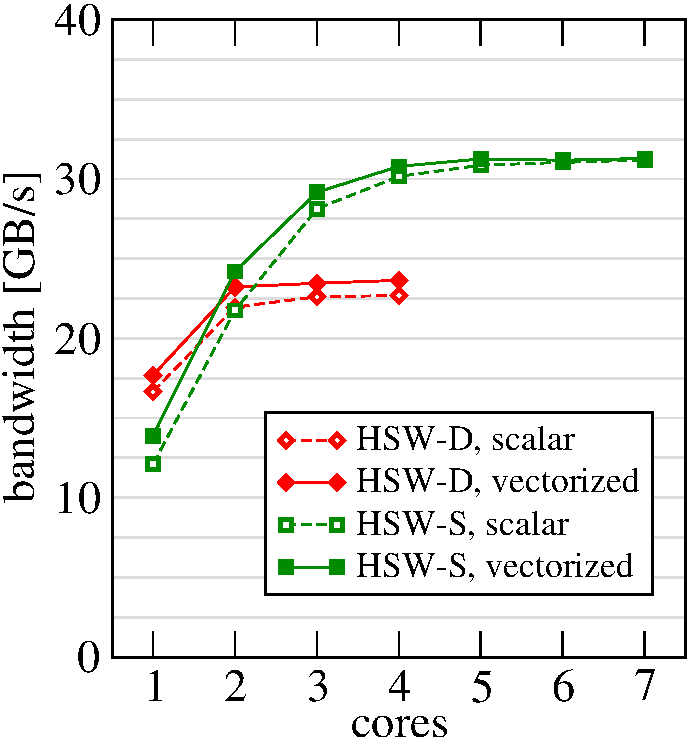
\includegraphics[height=0.4\linewidth,clip=true]{images/stream/StreamReadHswScalarVectorized}
    \label{fig:mrm:bw-scaling}
  } \, \hspace{0.5cm}
  \subfloat[]{%
    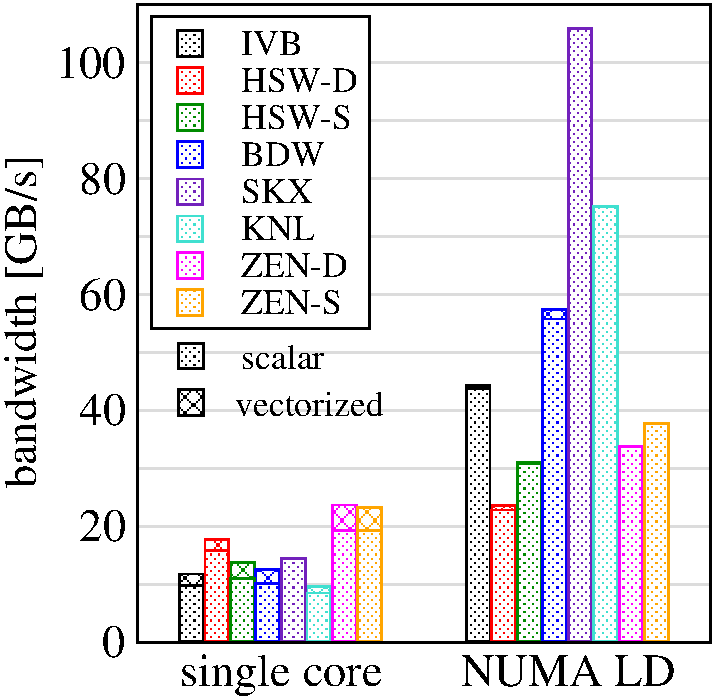
\includegraphics[height=0.4\linewidth,clip=true]{images/stream/StreamReadSingleCoreFullProcessor}
    \label{fig:mrm:bw-single-core}
  }%
  \caption{Bandwidth over the number of cores of the read only benchmark in a
scalar and vectorized version exemplified on HSW-D and
HSW-S~\protect\subref{fig:mrm:bw-scaling}.
Single core bandwidth and saturated bandwidth with all available cores of the
processor/cluster~\protect\subref{fig:mrm:bw-single-core}.}
  \label{fig:mrm:bw}
\end{figure}

The measured read-only bandwidth, required for the performance model, is
reported in Table~\ref{tab:hw}.
As discussed in Sect.~\ref{sec:mrm} only scalar loads are used.
%
If enough cores are used then scalar and vectorized read-only benchmarks
saturate the memory bandwidth with the only difference that the saturation of
the latter is already achieved with fewer cores. 
This is exemplified on HSW-D and HSW-S system shown in
Fig.~\ref{fig:mrm:bw-scaling}.
HSW-D and HSW-S show the typical saturation behavior for (current Intel) desktop
and server systems. 
Typically desktop systems nearly saturate the memory bandwidth with one core.
%
Figure~\ref{fig:mrm:bw-single-core} shows the difference between the scalar and
vectorized read-only benchmark for the single core and the usage of all cores
inside a NUMA LD over all systems in the test bed.
IVB, HSW-S, and the ZEN-based
systems reach,
with one core and vector loads between $15$\,\% and
$25$\,\%,
a higher bandwidth
than with scalar load instructions.
However, utilizing the full NUMA LD nearly no difference is visible.
%

% \subsection{Machine Balance $B_m$}
The machine balance $B_m$ from Table~\ref{tab:hw} considers the scalar read-only
memory bandwidths and the scalar double precision floating point capabilities of
the processors. 
This is either a scalar FMA or, if unavailable, a scalar addition and
multiplication for processing a nonzero.

%
% The code balance for sparse solve from from Tab.~\ref{tab:mrm:bc} when data
% resides in memory has in the best case its lowest value of $B_c = 4$\,B/F.
% This exceeds the machine balances of all systems in the test bed.
% According to the Roofline model, this indicates sparse solve is memory bound.

% The bandwidth between each cache level also shown in Table~\ref{tab:hw} is
% obtained from~\ref{intel-orm-2016}. 
% Despite the documentation reports $1$\,cy/cl between L1- and L2-cache for the
% Haswell microarchitecture, only around  half the bandwidth is observed to be
% reached~\cite{hofmann-2016-hsw}.
% Hence, we assume $2$\,cy/cl as bandwidth.
% vec faster than scalar in percent: (bw_vec / bw_scalar - 1) * 100
% ivb_emmy
% ["23.74"]
% bdw_broadep2
% ["17.94"]
% bdw_meggie
% ["7.78"]
% hsw_hasep1
% ["14.56"]
% knl_knightmare1
% ["12.64"]
% zen_summitridge1
% ["22.90"]
% zen_naples1
% ["20.44"]
% hsw_woody_hsw
% ["6.18"]
% sx_sxace
% ["0.00"]
% sks_skylakesp2
% ["-3.21"]


\subsection{Matrices}

% \begin{SCtable}[][t]
% %\begin{table}[tp]
%   \centering
%   \small
%   \begin{tabular}{ll|rrrrrr}
%   \hline
%          &&  \multicolumn{1}{c}{$\bm{n}$} &&
%             \multicolumn{1}{c}{$\bm{\text{nnz}(A)}$}  &&
%             \multicolumn{1}{c}{$\bm{\text{nnz}(L)}$}   \\ 
%   \hline
% % values for threads = 1, p = 80
%   dense  && $    20 \times 10^3$ && $200 \times 10^6$ &&  $  200 \times 10^6$  \\ % ps-n-20000-t-1-p-80
%   lapl1  && $   256 \times 10^3$ && $  3 \times 10^6$ &&  $  219 \times 10^6$  \\ % pl-n-40-b-4-t-1-p-80  N=40, B=4
%   lapl2  && $   343 \times 10^3$ && $  1 \times 10^6$ &&  $  166 \times 10^6$  \\ % pl-n-70-b-1-t-1-p-80  N=70, B=1
%   omen1  && $1\,751 \times 10^3$ && $ 32 \times 10^6$ && $1\,076 \times 10^6$  \\ % omen-rc2.5-lc160-t-1-p-80
%   omen2  && $   760 \times 10^3$ && $ 20 \times 10^6$ && $   690 \times 10^6$  \\ % omen-rc3.5-t-1-p-80
%   omen3  && $1\,271 \times 10^3$ && $ 42 \times 10^6$ && $1\,651 \times 10^6$  \\ % omen-rc4.5-t-1-p-80
%   bddc   && $   750 \times 10^3$ && $ 31 \times 10^6$ && $1\,590 \times 10^6$  \\ % mat\_Kii\_sd22\_size750141\_load2\_newton1
%   \hline
%   \end{tabular}
%   \caption{Dimension ($n$) and number of nonzeros ($\text{nnz}$) for $A$ and 
% $L$ for all benchmark matrices.}
%   \label{tab:m:list}
% % \end{table}
% \end{SCtable}


%In~Table~\ref{tab:m:list}, we present information on  
%the symmetric matrices which will be used
%for the performance modeling and experiments in the following sections.
Table~\ref{tab:m:list} lists matrix dimension ($n$), number of nonzeros in the
matrix ($\text{nnz}(A)$) and the factor (nnz$(L)$) of the matrices used for
benchmarking in the following sections.
% and the number of nonzeros in the factor ($\text{nnz}(L)$).
% It shows the matrix dimension ($n$), the number of nonzeros in the matrix ($\text{nnz}(A)$),  
% and the number of nonzeros in the factor ($\text{nnz}(L)$).
The reported numbers of nonzeros 
are reported for factorizations using single threaded execution
and a panel size $\panelsize = 80$. 
All matrices are sparse except 
for the first matrix \mymat{dense}, where both the matrix and  
the factor $L$ are dense. 
We use this dense matrix as a best case example for our single core performance
investigations.
The matrices \mymat{lapl1} and \mymat{lapl2} are test matrices arising from a
finite difference discretization of the Laplace operator in three dimensions
with Dirichlet boundary conditions. 
In addition, the matrix \mymat{lapl2} contains a block structure
of size $4$. 
The \mymat{omen} matrices correspond to a set of representative matrices from 
an atomistic nanoelectronic device engineering simulation code~\cite{luisier2011atomistic}. 
The matrix \mymat{bddc} arises from a finite element discretization of a typical
solid mechanics problem. Here, as a material model, a J2-elasto-plasticity model
was chosen and three-dimensional and piecewise quadratic tetrahedral finite
elements were used for the discretization. The matrix \mymat{bddc} represents a
typical subdomain problem arising in the BDDC (Balancing Domain Decomposition by
constraints) implicit finite element solver.

% \sout{Matrix \uwave{\mymat{bddc1}}
% \mycomment{OR: gemeint ist wohl BDDC; sollte doch mehr Information dazu hinein?
% FETI stimmt nicht, Referenz stimmt nicht}
% has been obtained from 
% \uwave{a finite element tearing and interconnecting (FETI)} code~\cite{klawonn2002dual}.
% Figure~\ref{fig:m:spy} shows the structure of $A$ for the different matrix
% classes.}
%, whereas more  interesting, is the nonzero distribution over the panel sizes of the factor $L$ found in 
%Figure~\ref{fig:m}.

Please note that the current factorization limits the number of parts to powers
of two.
To avoid load imbalance during the solve step we report results only for thread
counts which are powers of two.
%
%This leads to a load imbalance during the solve step, which is why in this
%article we only report results for thread counts which are equal to powers of
%two.

\begin{figure}[tp]
  \centering
  \captionsetup[subfigure]{farskip=0pt}%
  \subfloat[lapl]{%
    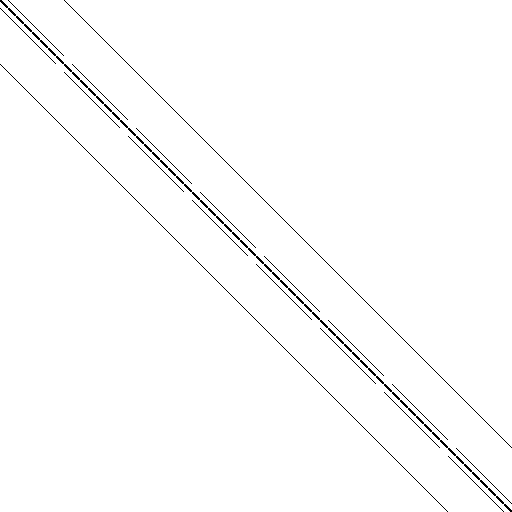
\includegraphics[width=0.25\linewidth,clip=true]{images/spy-plots/a-pl-n-8-b-1}
    \label{fig:m:spy:lp}
  }\,
  \subfloat[omen]{%
    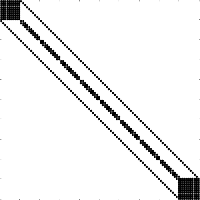
\includegraphics[width=0.25\linewidth,clip=true]{images/spy-plots/omen}
    \label{fig:m:spy:omen}
  }\,
  \subfloat[bddc]{%
    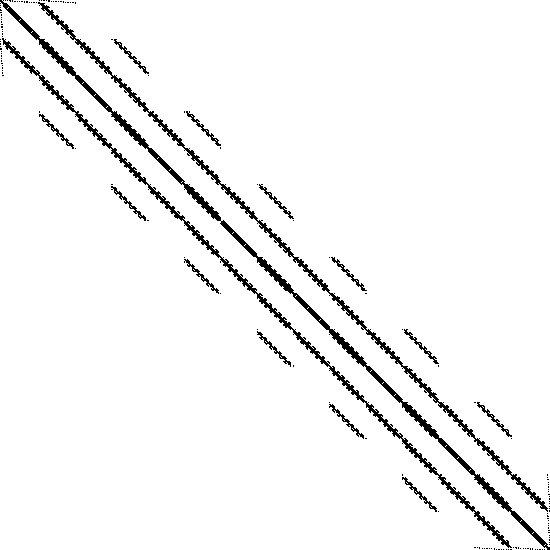
\includegraphics[width=0.25\linewidth,clip=true]{images/spy-plots/mat_Kii_sd89_size10992_load2_newton1}
    \label{fig:m:spy:feti}
  } 
  \caption{Structure of $A$ for matrix classes lapl~\protect\subref{fig:m:spy:lp},
  omen~\protect\subref{fig:m:spy:omen}, and bddc~\protect\subref{fig:m:spy:feti}.}
  \label{fig:m:spy}
\end{figure}

% {{{
% To generate/alter images:
% - go to directory data/matrices
%
% - run: ./plot-log.py <matrix-name>.dat
%   this will generate a pdf and png of the histogram.
%
% - copy the pdf to images/matrices
%
% \begin{figure*}[tp]
%   \centering
%   \subfloat[dense]{%
%     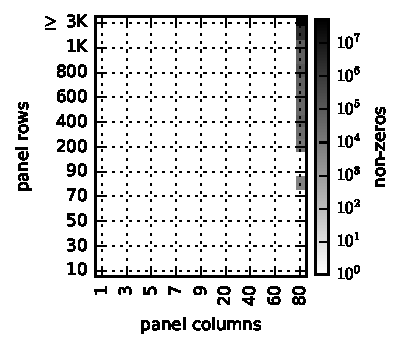
\includegraphics[width=0.3\textwidth,clip=true]{images/matrices/ps-n-20000-t-1-p-80}
%     \label{fig:m:dense}
%   } \,
%   \subfloat[lapl1]{%
%     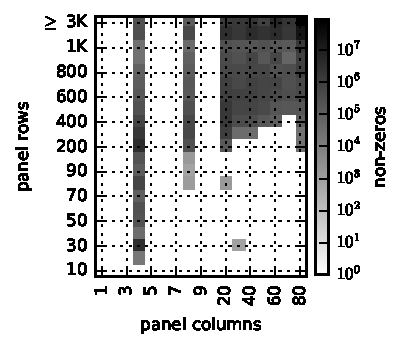
\includegraphics[width=0.3\textwidth,clip=true]{images/matrices/pl-n-00040-b-004}
%     \label{fig:m:laplace:n40b4}
%   } \,
%   \subfloat[lapl2]{%
%     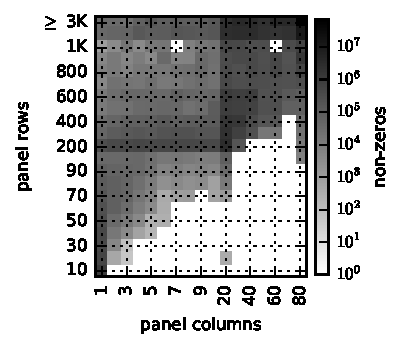
\includegraphics[width=0.3\textwidth,clip=true]{images/matrices/pl-n-70-b-1-t-1-p-80}
%     \label{fig:m:laplace:n70b1}
%   } \,
%   \subfloat[omen1]{%
%     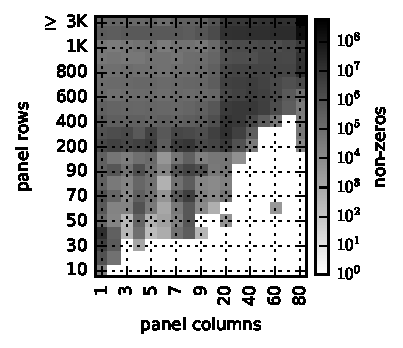
\includegraphics[width=0.3\textwidth,clip=true]{{{images/matrices/omen-rgf-tc2.5-lc160-t-1-p-80.hist-rhs-update-frequencies}}}
%     \label{fig:m:omen}
%   } \,
%   \subfloat[omen2]{%
%     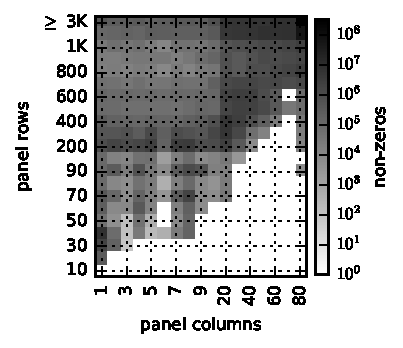
\includegraphics[width=0.3\textwidth,clip=true]{{{images/matrices/omen-rgf-tc3.5-t-1-p-80.hist-rhs-update-frequencies}}}
%     \label{fig:m:omen}
%   } \,
% %  \subfloat[omen3]{%
% %    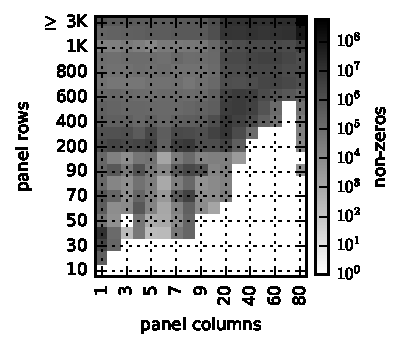
\includegraphics[width=0.3\textwidth,clip=true]{{{images/matrices/omen-rgf-tc4.5-t-1-p-80.hist-rhs-update-frequencies}}}
% %    \label{fig:m:omen}
% %  } \,
%   \subfloat[feti1]{%
%     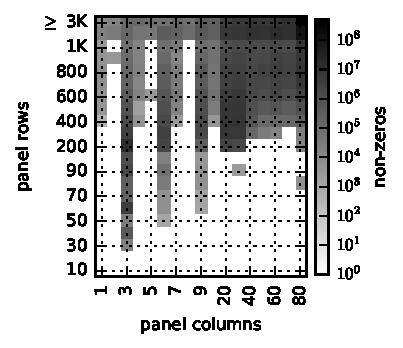
\includegraphics[width=0.3\textwidth,clip=true]{{{images/matrices/mat_Kii_sd22_size750141_load2_newton1-t-1-p-80.log-rhs-update-frequencies}}}
%     \label{fig:m:omen}
%   } \,
%   \caption{Multi-parameter histograms showing how many nonzeros of $L$ are in panels with a certain
%            number of columns and rows. Panels with $3000$ and more rows are
%            accumulated.
%            This plot gives an impression of how the work, i.e.,\ nonzeros,
%            in~$L$ is distributed over panel dimensions.
%   }
%   \label{fig:m}
% \end{figure*}
% }}}

\section{Performance Evaluation and Analysis}
\label{sec:pa}
\label{sec:performance}


For the code generation, we instruct
the compiler via directives to unroll the
innermost loops of Alg.~\ref{alg:algo:fw} and \ref{alg:algo:bw}, i.\,e.,
to perform an unrolling over the rows.
Here, an unrolling factor of eight or 16 showed the best
performance for all architectures.
%
We prohibit vectorization of this loops, which causes the
compiler to use scalar floating point addition/multiplication or FMA
instructions.
%
We observe that
%\mycomment{OR: Dies ist doch eine gewonnene Erkenntnis, oder? => We observe that}
with vectorization enabled for this loops the compiler
performs manual gather and scatter, which results in the same or even poorer
performance compared to the scalar unrolled versions.
This is required as AVX2 only includes a vector gather instruction.
%
Only for the 1-way column unrolling of sparse triangular solve
%\mycomment{OR: alle ``sparse solve'' durch ``forward/backward substitution'' ersetzen}
with KNL the compiler
generated loop utilizing vector scatter/gather instructions is superior to
the scalar version, which is why we use this version for the combination of KNL
and 1-way column unrolling.
However, also SKX supports vector gather/scatter instructions, but did not
show any performance improvement.

\begin{figure}[t]%
\centering%
\captionsetup[subfigure]{justification=centering,farskip=0pt}
\subfloat[][

IVB]{%
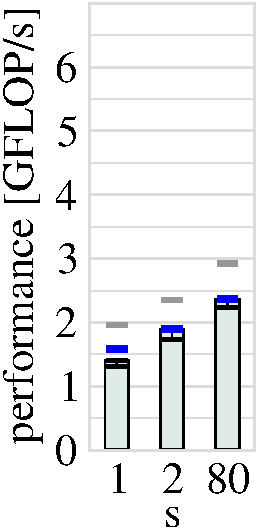
\includegraphics[height=2.9cm,clip=true]{images/perf/ps-n-20000/p-single-core-emmy-n-20000}
} %
\subfloat[HSW-D]{%
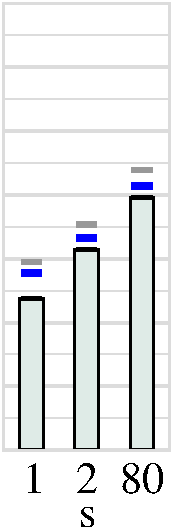
\includegraphics[height=2.9cm,clip=true]{images/perf/ps-n-20000/p-single-core-woody-hsw-n-20000}
} %
\subfloat[HSW-S]{%
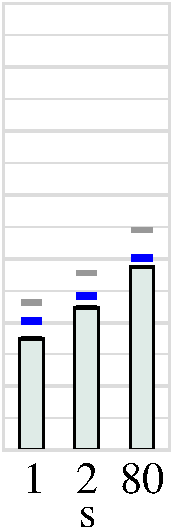
\includegraphics[height=2.9cm,clip=true]{images/perf/ps-n-20000/p-single-core-hasep1-n-20000}
} %
\subfloat[][

BDW]{%
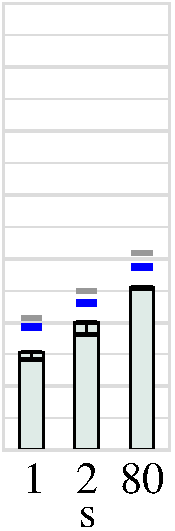
\includegraphics[height=2.9cm,clip=true]{images/perf/ps-n-20000/p-single-core-meggie-n-20000}
} %
\subfloat[][

SKX]{%
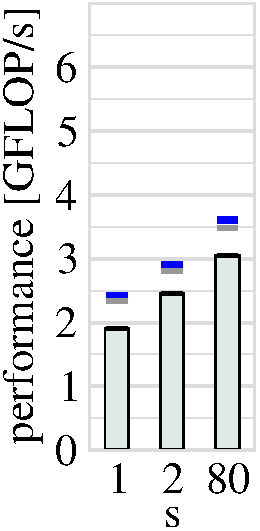
\includegraphics[height=2.9cm,clip=true]{images/perf/ps-n-20000/p-single-core-skylakesp2-n-20000}
} %
\subfloat[][

KNL]{%
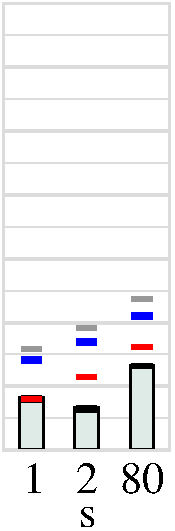
\includegraphics[height=2.9cm,clip=true]{images/perf/ps-n-20000/p-single-core-knightmare1-n-20000}
\label{fig:p:single-core:knl}
} %
\subfloat[ZEN-D]{%
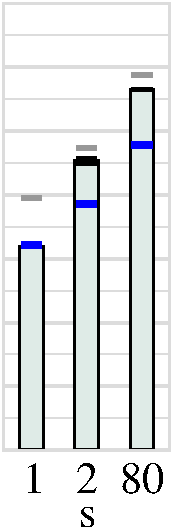
\includegraphics[height=2.9cm,clip=true]{images/perf/ps-n-20000/p-single-core-summitridge1-n-20000}
\label{fig:p:single-core:zen-d}
} %
\subfloat[ZEN-S]{%
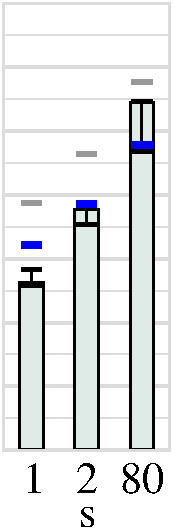
\includegraphics[height=2.9cm,clip=true]{images/perf/ps-n-20000/p-single-core-naples1-n-20000}
\label{fig:p:single-core:zen-s}
} %
  \caption{Performance of PARDISO's sparse triangular solve
    %with $1$-, $2$-, and $8$-way column unrolling 
    for matrix \mymat{dense}. % with panel size $\panelsize = 1$, $2$,
    %and $80$, respectively.
    Blue and gray horizontal bars show predictions of the modified Roofline model 
    with scalar and vectorized read bandwidth, respectively.
    }%
  \label{fig:p:single-core}%
\end{figure}

\begin{figure*}%
  \centering%
  
 \begin{tabular}{lcccccccc}
 %\begin{tabular}{>{\tiny \bfseries}lcccccccccc>{\tiny \bfseries}lccccccccccc}
 &
 \multicolumn{1}{c}{\tiny \bfseries IVB} & \multicolumn{1}{c}{\tiny \bfseries
HSW-D} & \multicolumn{1}{c}{\tiny \bfseries HSW-S} & \multicolumn{1}{c}{\tiny
\bfseries BDW} & \multicolumn{1}{c}{\tiny \bfseries SKX} &
\multicolumn{1}{c}{\tiny \bfseries KNL} & \multicolumn{1}{c}{\tiny \bfseries
ZEN-D} & \multicolumn{1}{c}{\tiny \bfseries ZEN-S} \\

% start matrix lapl1 (n-40-b-4)
 \raisebox{1.70cm}{\rotatebox[origin=c]{90}{lapl1}} &
  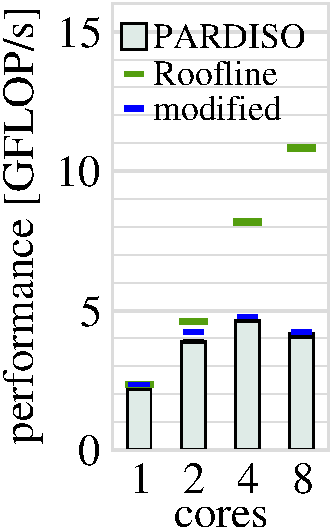
\includegraphics[height=3.0cm,clip=true]{images/perf/p-80/p-emmy-n-40-b-4}% 
  & 
  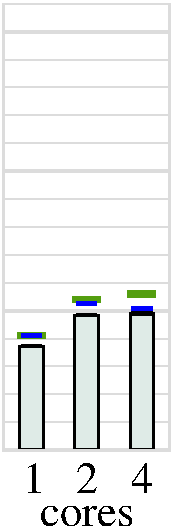
\includegraphics[height=3.0cm,clip=true]{images/perf/p-80/p-woody-hsw-n-40-b-4}% 
  & 
  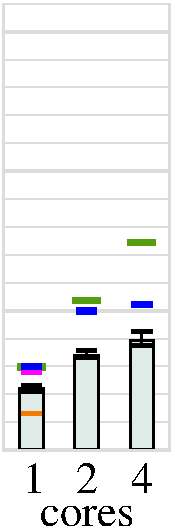
\includegraphics[height=3.0cm,clip=true]{images/perf/p-80/p-hasep1-n-40-b-4}% 
  & 
  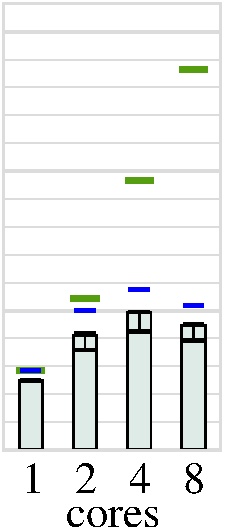
\includegraphics[height=3.0cm,clip=true]{images/perf/p-80/p-meggie-n-40-b-4}% 
  & 
  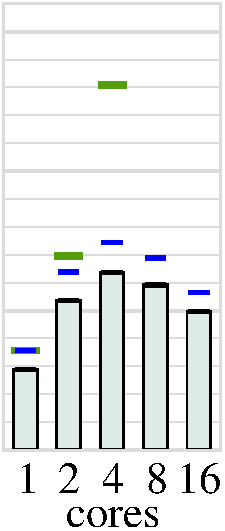
\includegraphics[height=3.0cm,clip=true]{images/perf/p-80/p-skylakesp2-n-40-b-4}% 
  & 
  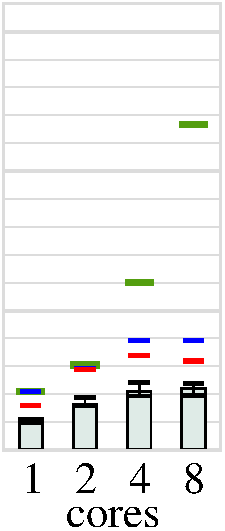
\includegraphics[height=3.0cm,clip=true]{images/perf/p-80/p-knightmare1-n-40-b-4}% 
  & 
  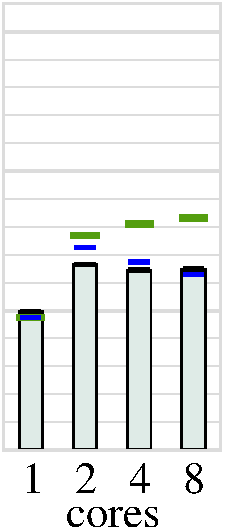
\includegraphics[height=3.0cm,clip=true]{images/perf/p-80/p-summitridge1-n-40-b-4}% 
  & 
  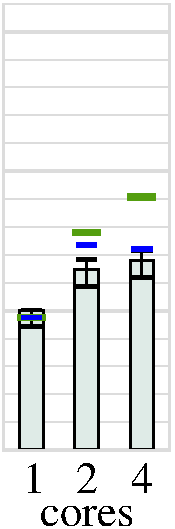
\includegraphics[height=3.0cm,clip=true]{images/perf/p-80/p-naples1-n-40-b-4}% 
%
\\
% end matrix n-40-b-4
% start matrix lapl2 (n-70-b-1)
 \raisebox{1.70cm}{\rotatebox[origin=c]{90}{lapl2}} &
  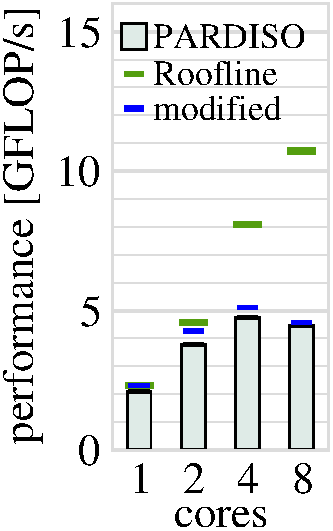
\includegraphics[height=3.0cm,clip=true]{images/perf/p-80/p-emmy-n-70-b-1}% 
  & 
  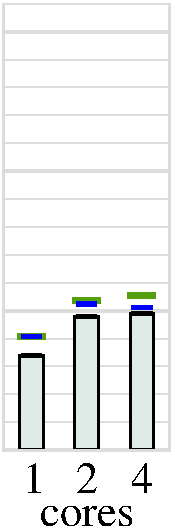
\includegraphics[height=3.0cm,clip=true]{images/perf/p-80/p-woody-hsw-n-70-b-1}% 
  & 
  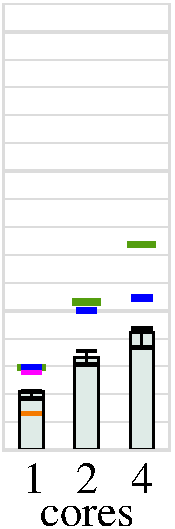
\includegraphics[height=3.0cm,clip=true]{images/perf/p-80/p-hasep1-n-70-b-1}% 
  & 
  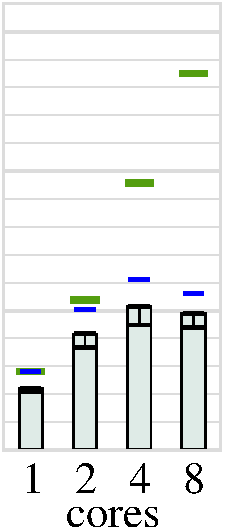
\includegraphics[height=3.0cm,clip=true]{images/perf/p-80/p-meggie-n-70-b-1}% 
  & 
  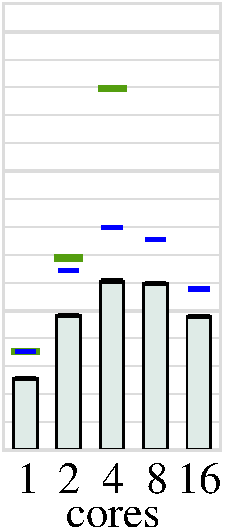
\includegraphics[height=3.0cm,clip=true]{images/perf/p-80/p-skylakesp2-n-70-b-1}% 
  & 
  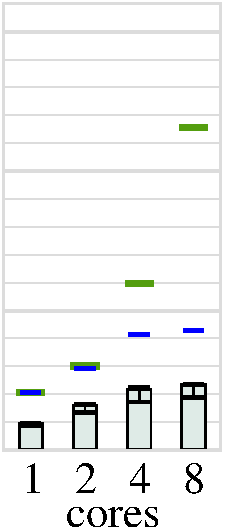
\includegraphics[height=3.0cm,clip=true]{images/perf/p-80/p-knightmare1-n-70-b-1}% 
  & 
  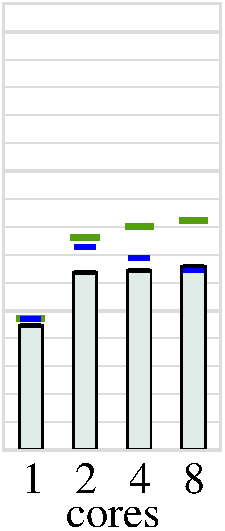
\includegraphics[height=3.0cm,clip=true]{images/perf/p-80/p-summitridge1-n-70-b-1}% 
  & 
  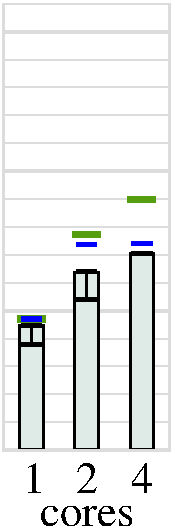
\includegraphics[height=3.0cm,clip=true]{images/perf/p-80/p-naples1-n-70-b-1}% 
\\
% end matrix n-70-b-1
% start matrix feti1 (mat_Kii_sd22_size750141_load2_newton1)
 \raisebox{1.70cm}{\rotatebox[origin=c]{90}{bddc1}} &
  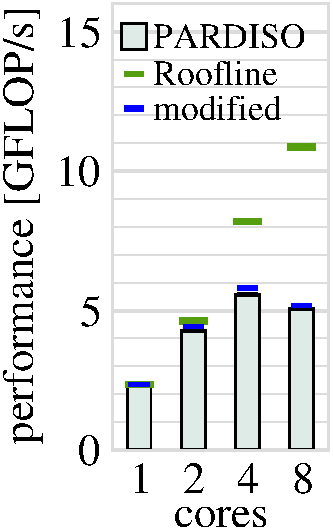
\includegraphics[height=3.0cm,clip=true]{images/perf/p-80/p-emmy-mat_Kii_sd22_size750141_load2_newton1}% 
  & 
  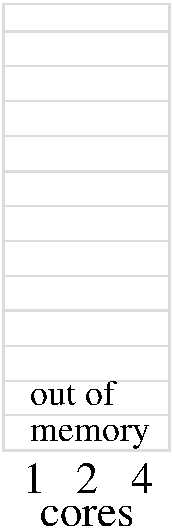
\includegraphics[height=3.0cm,clip=true]{images/perf/p-80/p-woody-hsw-mat_Kii_sd22_size750141_load2_newton1}% 
  & 
  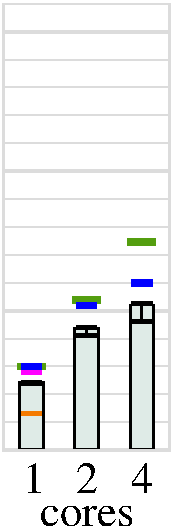
\includegraphics[height=3.0cm,clip=true]{images/perf/p-80/p-hasep1-mat_Kii_sd22_size750141_load2_newton1}% 
  & 
  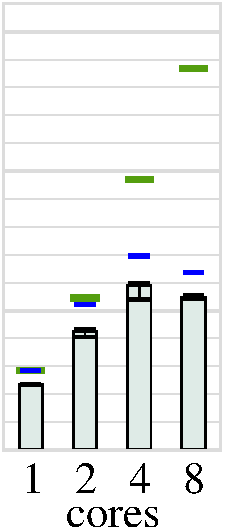
\includegraphics[height=3.0cm,clip=true]{images/perf/p-80/p-meggie-mat_Kii_sd22_size750141_load2_newton1}% 
  & 
  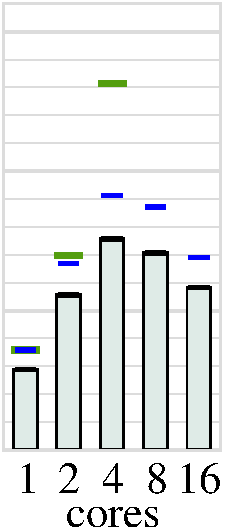
\includegraphics[height=3.0cm,clip=true]{images/perf/p-80/p-skylakesp2-mat_Kii_sd22_size750141_load2_newton1}% 
  & 
  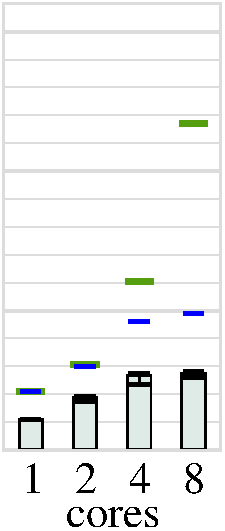
\includegraphics[height=3.0cm,clip=true]{images/perf/p-80/p-knightmare1-mat_Kii_sd22_size750141_load2_newton1}% 
  & 
  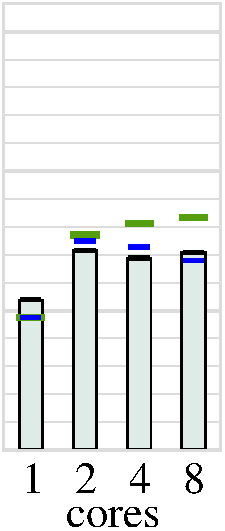
\includegraphics[height=3.0cm,clip=true]{images/perf/p-80/p-summitridge1-mat_Kii_sd22_size750141_load2_newton1}% 
  & 
  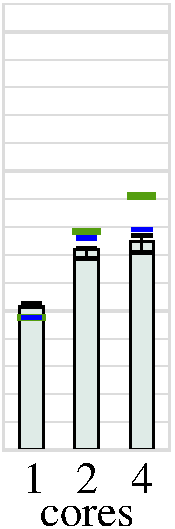
\includegraphics[height=3.0cm,clip=true]{images/perf/p-80/p-naples1-mat_Kii_sd22_size750141_load2_newton1}% 
\\



% &
% \multicolumn{1}{c}{\tiny \bfseries IVB} & \multicolumn{1}{c}{\tiny \bfseries
%HSW-D} & \multicolumn{1}{c}{\tiny \bfseries HSW-S} & \multicolumn{1}{c}{\tiny
%\bfseries BDW} & \multicolumn{1}{c}{\tiny \bfseries SKX} &
%\multicolumn{1}{c}{\tiny \bfseries KNL} & \multicolumn{1}{c}{\tiny \bfseries
%ZEN-D} & \multicolumn{1}{c}{\tiny \bfseries ZEN-S} \\

% start matrix lapl1 (n-40-b-4)
\raisebox{1.70cm}{\rotatebox[origin=c]{90}{omen1}} &
  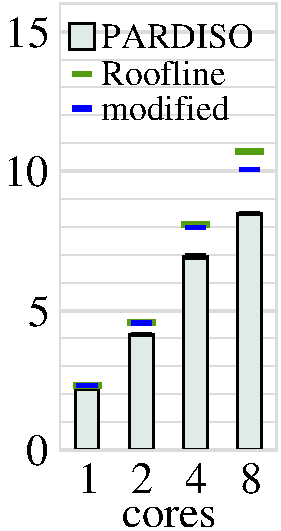
\includegraphics[height=3.0cm,clip=true]{images/perf/p-80/p-emmy-omen-rgf-tc2_5-lc160}% 
  & 
  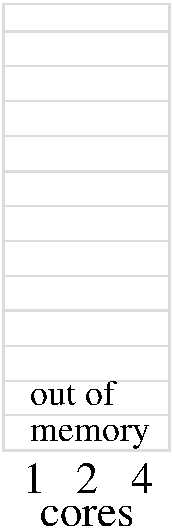
\includegraphics[height=3.0cm,clip=true]{images/perf/p-80/p-woody-hsw-omen-rgf-tc2_5-lc160}% 
  & 
  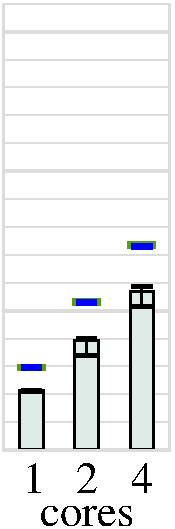
\includegraphics[height=3.0cm,clip=true]{images/perf/p-80/p-hasep1-omen-rgf-tc2_5-lc160}% 
  & 
  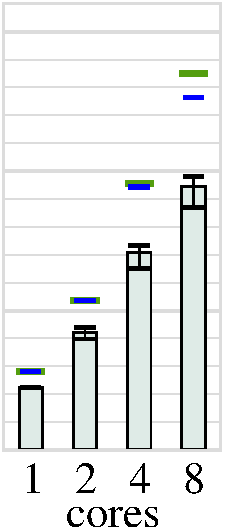
\includegraphics[height=3.0cm,clip=true]{images/perf/p-80/p-meggie-omen-rgf-tc2_5-lc160}% 
  & 
  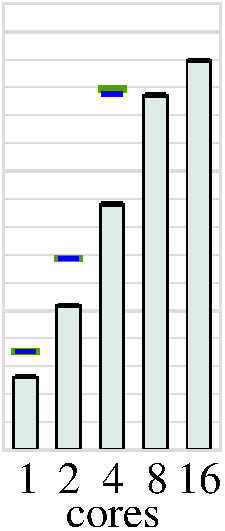
\includegraphics[height=3.0cm,clip=true]{images/perf/p-80/p-skylakesp2-omen-rgf-tc2_5-lc160}% 
  & 
  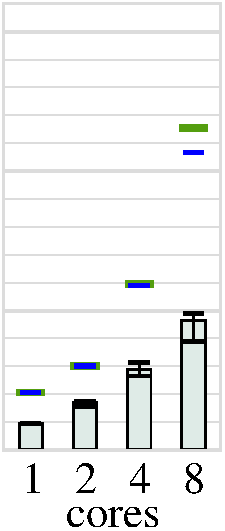
\includegraphics[height=3.0cm,clip=true]{images/perf/p-80/p-knightmare1-omen-rgf-tc2_5-lc160}% 
  & 
  \includegraphics[height=3.0cm,clip=true]{images/perf/p-80/p-summitridge1-omen-rgf-tc2_5-lc160}% 
  & 
  \includegraphics[height=3.0cm,clip=true]{images/perf/p-80/p-naples1-omen-rgf-tc2_5-lc160}% 
\\
% end matrix n-40-b-4
% start matrix lapl2 (n-70-b-1)
\raisebox{1.70cm}{\rotatebox[origin=c]{90}{omen2}} &
  \includegraphics[height=3.0cm,clip=true]{images/perf/p-80/p-emmy-omen-rgf-tc3_5}% 
  & 
  \includegraphics[height=3.0cm,clip=true]{images/perf/p-80/p-woody-hsw-omen-rgf-tc3_5}% 
  & 
  \includegraphics[height=3.0cm,clip=true]{images/perf/p-80/p-hasep1-omen-rgf-tc3_5}% 
  & 
  \includegraphics[height=3.0cm,clip=true]{images/perf/p-80/p-meggie-omen-rgf-tc3_5}% 
  & 
  \includegraphics[height=3.0cm,clip=true]{images/perf/p-80/p-skylakesp2-omen-rgf-tc3_5}% 
  & 
  \includegraphics[height=3.0cm,clip=true]{images/perf/p-80/p-knightmare1-omen-rgf-tc3_5}% 
  & 
  \includegraphics[height=3.0cm,clip=true]{images/perf/p-80/p-summitridge1-omen-rgf-tc3_5}% 
  & 
  \includegraphics[height=3.0cm,clip=true]{images/perf/p-80/p-naples1-omen-rgf-tc3_5}% 
\\
% end matrix n-70-b-1
% start matrix feti1 (mat_Kii_sd22_size750141_load2_newton1)
\raisebox{1.70cm}{\rotatebox[origin=c]{90}{omen3}} &
  \includegraphics[height=3.0cm,clip=true]{images/perf/p-80/p-emmy-omen-rgf-tc4_5}% 
  & 
  \includegraphics[height=3.0cm,clip=true]{images/perf/p-80/p-woody-hsw-omen-rgf-tc4_5}% 
  & 
  \includegraphics[height=3.0cm,clip=true]{images/perf/p-80/p-hasep1-omen-rgf-tc4_5}% 
  & 
  \includegraphics[height=3.0cm,clip=true]{images/perf/p-80/p-meggie-omen-rgf-tc4_5}% 
  & 
  \includegraphics[height=3.0cm,clip=true]{images/perf/p-80/p-skylakesp2-omen-rgf-tc4_5}% 
  & 
  \includegraphics[height=3.0cm,clip=true]{images/perf/p-80/p-knightmare1-omen-rgf-tc4_5}% 
  & 
  \includegraphics[height=3.0cm,clip=true]{images/perf/p-80/p-summitridge1-omen-rgf-tc4_5}% 
  & 
  \includegraphics[height=3.0cm,clip=true]{images/perf/p-80/p-naples1-omen-rgf-tc4_5}% 
\\


% end matrix omen-rgf-tc4.5
% &
%&\tiny \makecell{$e = $ \\ $[-1, 18 ]$}&\tiny \makecell{$e = $ \\ $[0, 19 ]$}&\tiny \makecell{$e = $ \\ $[15, 51 ]$}&\tiny \makecell{$e
%= $ \\ $[14, 33 ]$}&\tiny \makecell{$e = $ \\ $[13, 62 ]$}&\tiny \makecell{$e = $ \\ $[59, 129 ]$}&\tiny \makecell{$e = $ \\ $[-11, 17
%]$}&\tiny \makecell{$e = $ \\ $[-7, 28 ]$}
%
%&&
%
% &
%&\tiny \makecell{$e = $ \\ $[-1, 18 ]$}&\tiny \makecell{$e = $ \\ $[0, 19 ]$}&\tiny \makecell{$e = $ \\ $[15, 51 ]$}&\tiny \makecell{$e
%= $ \\ $[14, 33 ]$}&\tiny \makecell{$e = $ \\ $[13, 62 ]$}&\tiny \makecell{$e = $ \\ $[59, 129 ]$}&\tiny \makecell{$e = $ \\ $[-11, 17
%]$}&\tiny \makecell{$e = $ \\ $[-7, 28 ]$}
\end{tabular}
%
%
  %
  \caption{Performance of sparse triangular solve with benchmark matrices of
panel size $s=80$ on one NUMA LD for each hardware system.
  Green and blue bars show predictions of the original and modified Roofline
model, respectively.
  HSW-S and ZEN-S have 14 and 24 cores in total and using all cores could
achieve with correct NUMA placement a higher performance, respectively. 
  Bottom row shows the model error $e$ for the corresponding system in
percent.}%
  \label{fig:p:pardiso}
\end{figure*}

For the single core measurements we use the matrix \mymat{dense}.
We create three variants of it, where the maximum panel size $\panelsize$ is
limited to $1$, $2$, and $80$ columns.
This enables isolated measurement of the $1$-, $2$-, and $8$-way
unrolled loops.
Furthermore, matrix \mymat{dense} exhibits the most homogeneous access pattern
as memory is only accessed in long contiguous streams and relates best to our
read-only benchmark (Sect.~\ref{sec:tb:membw}) used as input for the modified
Roofline model (Sect.~\ref{sec:mrm}, \eqref{eq:rm:mod}).
%
Figure~\ref{fig:p:single-core} shows the measured performance for all systems in
our testbed for sparse triangular solve.
The blue bars indicate the performance limit from the modified Roofline model.
%
In general larger panels deliver a higher performance.
This is expected as the code balance decreases with increasing panel sizes.
For panel size $s=1$ and $s=2$ with matrix \mymat{dense} the worst case code balance
of $B_c=6$\,B/F and $B_c=5$\,B/F is reached, respectively. 
With a panel size $s=80$ the code balance for the $8$-way unrolled loop nearly
becomes $B_c=4$\,B/F.
  
The modified Roofline model predictions for the Intel based systems (except for
KNL) deviate up to $25$\,\% from the measurements, but achieve a higher
performance with larger panels.
%
For KNL the model error is in the range of $55$\,\% to $160$\,\% over all panel
sizes which suggests some error in the model assumptions.
On KNL a STREAM like (scalar) copy and read benchmark achieves a L2 bandwidth of
around $7.8$\,GB/s and $8.5$\,GB/s with one core,
respectively.
From Fig.~\ref{fig:ecm:data}, we see that between L1 and L2 cache (depending on
the matrix) we might have a higher code
balance compared to the one we assume between memory and L2.
As the measured L2 bandwidth is nearly equal to the memory read-only bandwidth
the former data path becomes the new bottleneck.
However, determining a priori the code balance between L1 and L2 cache for a matrix
is analytically nontrivial, why we derive the metric from the measured data
traffic between the caches.
The adjusted model based on this new inputs is shown in
Fig.~\ref{fig:p:single-core:knl} as red bars and reduces the model error
significantly.
%
The poor performance with panel size $s = 2$ however, is unclear and deserves
further investigation. 
%
%
% The measured data traffic between memory and L2 is only about $5$\,\% higher
% than our model assumption for $s=1$ and $s=2$.
% With $s=80$ we measure a $25$\,\% increased amount of data.
% Despite the latter deviation is pretty large the increased memory traffic cannot
% (alone) account for the performance discrepancy on KNL.
% Currently we are still investigating this issue.
% \todo{multi stream?}
%
The Roofline model for the AMD based ZEN systems underestimates the
performance by up to $20$\,\%.
It seems that sparse solve in case of ZEN-D and $s=2, 80$ and ZEN-S and $s=80$
achieves the bandwidth obtained with the vectorized read benchmark as the bars
in Fig.~\ref{fig:p:single-core:zen-d} and~\ref{fig:p:single-core:zen-s} match
the gray lines, which represent the modified Roofline model based on the
vectorized read-only bandwidth.
Measuring the actual clock frequency shows that ZEN-D and ZEN-S run with
$3.8$\,GHz and $3.2$\,GHz during sparse solve, respectively.
However, they also achieve this frequency during read-only bandwidth
measurements.
Until now its unclear why both systems reach a higher bandwidth with sparse
solve compared to the scalar read only benchmark.
% \todo{multi stream not the answer}
% As we are currently unable to measure the memory traffic on this architecture
% we cannot compare it to our model assumptions we have to postpone further
% investigations regarding this issue.
% \todo{only scalar FMA used}
%
%1 For the SX machine the modified Roofline model predictions exceed the graphs
%1 y-axis and are therefore not shown.
%1 As expected due to the high single core bandwidth the SX ACE outperforms all
%1 other machines.
% As the compiler already utilizes gather and scatter instructions and places
% vector $r$ in the ADB (assignable data buffer, a $1$\,MiB large vector cache) in
% both code versions, we did not explicitly include any other optimizations.

%%%%%%%%%%%%%%%%%%%%%%%%%%%%%%%%%%%%%%%%%%%%%%%%%%%%%%%%%%%%%%




Performance results for all matrices are shown in Fig.~\ref{fig:p:pardiso}.
For HSW-D (second column) the main memory was not large enough for benchmarks
with the \mymat{bddc}, \mymat{omen2}, and \mymat{omen3} matrices, which is
indicated as ``out of memory'' in the figures.
%
%
Currently we only can ensure correct NUMA placement for one locality domain, why
we limit the scope of the analysis to one NUMA LD only. 
Hence, for HSW-S and ZEN-S less cores than the processor houses are used.
Please keep in mind, that for HSW-S seven of 14 cores and for ZEN-S only six of
24 cores are used and with correct NUMA placement and usage of more cores a
higher performance could be achieved.

\begin{SCfigure}[2][t]%
%\begin{figure}[t]%
  \centering%
  \includegraphics[width=0.25\textwidth,clip=true]{images/matrices-serial-fraction}%
  \caption{Fraction of nonzeros in the separator, which must be processed
   serially, depending on the number of cores for test matrices.  }%
  \label{fig:p:serial-fraciton}%
%\end{figure}
\end{SCfigure}

As already pointed out, the number of independent parallel parts produced by the
factorization is always a power of two.
For non-power of two thread counts this results in load imbalance and decreases
performance, why we omit them in the graphs.
%
Furthermore, the current implementation of the factorization increases the size
of the separator in the factor $L$ with increasing number of threads as already
observed in scaling studies for sparse solve in~\cite{klawonn-2015}.
%
Figure~\ref{fig:p:serial-fraciton} shows the fraction of nonzeros in $L$ which are
part of the separator, i.\,e.\ the part which must be executed serial.
Except for \mymat{omen1} this prohibits the efficient usage of larger core
counts and the test matrices reach their highest performance already with four
or eight cores.
%
This is also the reason why we cannot efficiently utilize KNL's high bandwidth
memory.
Despite its bandwidth scales (nearly) linearly with the number of cores its
single core bandwidth is not significantly different to the one delivered from
main memory.
Only with higher core counts the full HBM bandwidth can be obtained.
However, with $16$, $32$, and $64$ threads the serial fraction of the resulting
factor from the matrices is already to high and performance nearly drops to
the single core performance level.
Hence, we excluded HBM measurements from the plots as it gives no further
insight.
%
With SKX hosting $20$ cores in one NUMA LD the impact of the separator becomes
visible (fifth column of Fig.~\ref{fig:p:pardiso}).
The separator of \mymat{lapl1}, \mymat{lapl2}, and \mymat{bddc}\/ strongly increases 
over the number of cores and limits the scaling of the performance early.
The maximum performance here is already reached with four cores.
The increase of the serial fraction for \mymat{omen2} and \mymat{omen3} is not
that pronounced.
Here, the performance peak is reached with eight cores.
Only with \mymat{omen1}, where the separator stays small, performance increases
up to 16~cores.
All other architectures follow this pattern up to the number of cores used.

Figure~\ref{fig:p:pardiso} also shows the performance limits for the original
\eqref{eq:rm:simple} and the modified Roofline model \eqref{eq:rm:mod}
as green and blue bars, respectively.
As the traditional model misses the serial fraction of the execution it scales
with the achievable bandwidth of the number of cores used.
This is increasingly pronounced, the larger the serial fraction becomes. 
%The gap between the models depends on two factors.
%Firstly the amount of the serial fraction of the matrix and secondly the ratio
%between the achievable memory bandwidth of the used cores compared to the single
%core bandwidth.
%
Systems saturating with one core nearly the total memory bandwidth exhibit
only a marginally gap, like HSW-D (second column in Fig.~\ref{fig:p:pardiso}) or
slightly more pronounced ZEN-D (seventh column in Fig.~\ref{fig:p:pardiso}).

In general the modified Roofline model captures the behavior of the measured
performance over all systems and matrices as Fig~\ref{fig:p:pardiso} shows.
%
%
IVB and HSW-D, ZEN-D, and ZEN-S exhibit a model error of around $20$\,\% shown
in the bottom row of Fig.~\ref{fig:p:pardiso}. 
For HSW-S, BDW, and SKX the model deviates up to $60$\,\% from the measurements.
%
% Especially the predictions for the \mymat{omen} matrices are around $10$\,\%
% worse than for the other matrices.
%
As measured data traffic is in the expected bounds a deeper analysis of the
architectures and algorithm is required.
One option for future investigations is the ECM performance
model~\cite{hager-2012-ecm}, which not only accounts for all transfers inside
the memory hierarchy but also performs an in-depth analysis of the execution in
the core.
%
%
For KNL the bottleneck with multiple cores becomes more complex than with a
single core.
The L2 bandwidth scales linearly with each core, whereas the memory bandwidth
scales only with pairs of cores, i.\,e.\ per tile, and saturates at a certain
point.
Depending on the matrix and the size of its separator L2 or memory bandwidth can
now be the bottleneck.
%
In order to keep the model simple, for KNL, we show
as red bars in Fig.~\ref{fig:p:pardiso},
in addition
to the modified
Roofline model, 
an adjusted version; cf.\ the single core measurements.
Here, we consider \mymat{lapl1} and \mymat{omen2}.
Note that all measurements might suffer from the poor performance of $2$-way
column unrolling.
%
% limited by shows the same behavior as with one core and matrix \mymat{dense}.
% Its performance stays far behind the predictions.
% 
HSW-D and ZEN-D nearly can saturate the memory bandwidth with one core and gain
nearly no benefit from using more than two cores.

% The gray lines in Fig.~\ref{fig:p:pardiso} show the modified Roofline model
% based on the vectorized read-only bandwidth. \todo{vectorization} 
% \todo{potential of vectorization}








%\todop{
%\begin{itemize}
%    \item Describe CPU
%    \item Vectorization (AVX)
%    \item NUMA
%    \item What else?
%    \item 
%    \item Tools to get information about CPU / memory
%    \item /proc/cpuinfo, /proc/meminfo
%    \item hwloc, likwid
%    \item 
%    \item Profilers?
%    \item likwid
%    \item 
%    \item likwid paper: \cite{likwid-2010}
%\end{itemize}
%}
%
%\todol{some introduction}
%According to Moore's law, performance of processors double every eighteen months.
%For many years the performance was increased by increasing the clock speed of the CPU. This was very convenient because programmers could achieve the speedup with no effort, simply by buying a newer generation of CPU.
%\todol{no free lunch}
%However, the clock speed cannot keep increasing forever. Increasing frequency inevitably increases power consumption \todol{this is nonlinear}, which comes hand in hand with higher demand for cooling. While higher power consumption is not necessarily a problem for server or cluster installations, overheating becomes the real problem.
%
%Another way of increasing performance is adding more transistors on the chip \todol{this is linear}, which allows executing more computations at the same time.
%There are two ways of implementing the parallelism. first option is implementing another unit called core, that can independently perform any operations. \todol{easy solutions for multitasking, for one process requires synchronization of memory accesses}
%
%Second options is implementing instructions that perform more than one arithmetical operation. This can either be performing the same operation on more operands at once, so called vector instructions (SSE, AVX), or performing more operations with the same operands. Multiplication and addition is often combined in one instruciton called fused multiply-add (FMA).
%These two approaches can also be combined to compute FMA operation on vector of data (AVX2).
%
%Increasing computational power allows processing need to be stored somewhere. In 1980s computers were quipped with kilobytes of memory while today's computers have gigabytes or even terabytes or memory. 
%
%\todop{memory size}
%
%\begin{itemize}
%    \item Increase performance: more cores or more operations in one instruction (vector instructions). Mention Moore's law.
%    \item 
%    \item CPU instructions work with data in registers (fast, but small memory placed in the CPU)
%    \item Main memory is big (GB - TB), but accessing it takes long time
%    \item To speed up the memory access, there is a cache between CPU and main memory. Usually there are three cache levels called L1, L2 and L3. L1 cache is smallest and closest to the CPU, L3 is largest and close to the memory.
%    \item When CPU accesses a memory, it calls a load instruction. \todol{checks TLB, if found (cache hit), loads the data, if not found (cache miss), loads data from lower cache level or main memory, this may require evicting other data from cache to free space}
%    \item 
%    \item 
%    \item 
%    \item 
%    \item 
%    \item 
%    \item 
%    \item 
%    \item 
%\end{itemize}